% LaTeX source for ``Complexity and Computation''
% Copyright (c)  2011  Allen B. Downey.

% Permission is granted to copy, distribute, transmit and adapt
% this work under a Creative Commons
% Attribution-NonCommercial-ShareAlike 3.0 Unported License:
% http://creativecommons.org/licenses/by-nc-sa/3.0/

% If you are interested in distributing a commercial version of this
% work, please contact Allen B. Downey.

% The LaTeX source for this book is available from
% http://greenteapress.com/complexity
% http://code.google.com/p/complexity

% This book was typeset using LaTeX .  The illustrations were
% drawn in xfig.  All of these are free, open-source programs.

%%----------------------------------------------------------------

% How to compile this document:
% If your environment provides latex, makeindex, and dvips,
% the following commands should produce a Postscript version
% of the book.

%        latex book
%        makeindex book
%        latex book
%        dvips -o book.ps book

% You will also need the following (fairly standard) latex
% packages: url, epsfig, makeidx, fancyhdr

% This distribution also includes a Makefile that should
% compile both the Postscript and PDF versions of the book.

%%-----------------------------------------------------------------

\documentclass[10pt]{book}
%\pdfminorversion=5
%\pdfobjcompresslevel=2

\usepackage[width=5.5in,height=8.0in,
  hmarginratio=3:2,vmarginratio=1:1]{geometry}

\usepackage[T1]{fontenc}
\usepackage{textcomp}
\usepackage{mathpazo}

\usepackage{url}
\usepackage{fancyhdr}
\usepackage{graphicx}
\usepackage{amsmath, amsthm, amssymb}
\usepackage{exercise}
\usepackage{makeidx}
\usepackage{setspace}
\usepackage{hevea}
\usepackage{verbatim}
\usepackage{upquote}

\newcommand{\thetitle}{Think Complexity}
\newcommand{\theversion}{1.2.2}

\title{\thetitle}
\author{Allen B. Downey}

% these styles get translated in CSS for the HTML version
\newstyle{a:link}{color:purple;}
\newstyle{p+p}{margin-top:1em;margin-bottom:1em}
\newstyle{img}{border:0px}


\makeindex

\newtheorem{exercise}{Exercise}[chapter]

\begin{document}



\chapter{Case study: Zipf's Law and Music}

{\em Max Ward (20748588)}

\section{Music as Language}

Zipf's law was introduced in Chapter 5. To recapitulate, it posits that the frequency of a word is inversely proportional to its rank. The rank of a word being defined as its index in a frequency table. The canonical example of this is the words of long piece of literature, usually a novel. It is a classical example of a scale-free distribution, and is defined by $f = r^{-a}$ where $f$ is frequency and $r$ is rank. A frequency distribution is said to be Zipfian if $a \approx 1$. Because of this, when plotted on a log-log scale (equivalent to taking the log of both sides), a Zipfian distribution appears to be a line with slope $m \approx -1$. Though Zipf's law is typically described in terms of novels, and thus written language, it actually refers to any natural language. Natural language is generally regarded to be any non-contrived language---which is to say that its use and invention is unpremeditated. Clearly most written and spoken languages are natural languages, however, written and performed music is also a type of natural language.

Figure of a log log zipf graph here

Music, among other art forms, is often regarded as communication. Like other forms of human communication it has structure and rules. While I shall not give a formal definition of these, the reader may refer to \url{http://en.wikipedia.org/wiki/Music_theory} for a concise overview. This chapter investigates Zipf's law in music. This is done using the MIDI file type, which is a relatively simple and widely used way to encode music digitally.


\begin{exercise}

There are specific parts of the human brain involved in language. For example, damage to Broca's area can profoundly affect ones ability to understand spoken and written language. Does an analogous region exist for processing music? (Hint: try searching for `Amusia'.)

\end{exercise}

\section{The MIDI Format}

The MIDI file format comprises a header and a series of one or more tracks. Ever MIDI track also contains a header, which is followed by a sequence of events. There are many event types which refer to any time related possibility. However, the only two which we consider in this investigation are the `Note On' and `Note Off' events. A Note On event has a time, a velocity, and a note. The time is when it is played, the velocity is the force with which it is played, and the note is the specific sound frequency of the event. It should be noted that velocity is not volume. It is possible than a MIDI instrument could have a linear velocity-volume relationship, but it could be exponential, logarithmic, or anything else. There are 128 distinct notes in the MIDI format, these are analogous to an extended piano (which has only 88 keys), with each increment indicating a semitone increase in sound frequency.

Figure of a piano keyboard here.

Parsing the MIDI file format can be difficult, as such, it is often relegated to a library. Python does not come with an easy to install MIDI parsing library. However, an open source effort called \texttt{python-midi} is available on Github under the MIT licence. It can be found here \url{https://github.com/vishnubob/python-midi}. Download or clone the repository and use the source files in your project. Once they are in the same folder, you should be able to import them like any Python library. I have provided a basic example that loads a MIDI file, given a file name from the command line. The \texttt{fileio} module is part of \texttt{python-midi}. It contains functions related to reading and parsing MIDI files.


\begin{verbatim}
import sys
import fileio


def main(name, fname, *args):
    pattern = fileio.read_midifile(fname)
    print pattern


if __name__ == '__main__':
    main(*sys.argv)

\end{verbatim}


The way MIDI patterns are represented in \texttt{python-midi} is straightforward. A pattern is a list of tracks. A track is a list of events. Every event has a type, and associated meta-data. All of these classes also have the \texttt{\_\_repr\_\_} method overloaded. This makes it easy to determine what information is available. A quirk of some older MIDI files is that a Note On event with velocity 0 is equivalent to the corresponding Note Off event. Keep this in mind when experimenting with MIDI files.

The Classical Archive has some excellent MIDI encodings of classical music (available at \url{http://www.classicalarchives.com/midi.html}). You may also wish to find some songs which you enjoy, many people have made their MIDI versions of songs freely available on the Internet. There is also software that allows the user to write MIDI music using a graphic environment. If you are so inclined, it is possible to analyse your own compositions.


\begin{exercise}
Research the MIDI format. How hard do you think it would be to write your own parser? Remember, if you improve \texttt{python-midi}, submit a pull request to Github!
\end{exercise}

\begin{exercise}
Attempt to write a script that outputs the number of distinct notes in a MIDI file. My solution is available at URL.
\end{exercise}


\section{Words and Music}

Zipf's law refers to the frequency of words found in a large corpus of natural language. It is hard to see how the concept of a word could apply to musical compositions. Of course, any interpretation of a word in music is necessarily arbitrary and somewhat open to interpretation. Despite this, I shall now describe several feasible candidates. Clearly the most obviously irreducible component of a musical composition is the note. Building upon this starting point, one might analyse the velocities, lengths, or the spacing between similar notes. More complex interpretations may attempt to group notes into structures like chords or melodies. I shall, however, start with a much simpler interpretation.

\subsection{Note Groupings}
\label{sec:note_group}
As I have said, we can break a piece of music up into notes. If we define a word as a single note, we can then collect the frequencies of these notes, and thence subject them to Zipfian analysis. This necessitates going through every MIDI event in every MIDI track for any given pattern. The \texttt{python-midi} package makes this quite easy, as tracks and events are represented as objects that inherit from \texttt{list}. Here is a simple function that returns all the notes (in no particular order) given the path to a MIDI file.

\begin{verbatim}
def get_notes(fname):
    pattern = fileio.read_midifile(fname)
    notes = []
    for track in pattern:
        for event in track:
            if event.name == "Note On" and event.data[1] > 0:
                notes.append(event.data[0])
    return notes
\end{verbatim}

The first line reads and parses the MIDI into a pattern. The follow two loops examine every event in the pattern. Every time a genuine Note On event is spotted (remember that a Note On event with velocity 0 is actually a Note Off event) it is added to the \texttt{notes} list. It should be pointed out that event data is stored in the \texttt{event.data} member. For Note On events, index zero is the MIDI note, and index one is the velocity. After executing this function, we now have everything we need to calculate frequency as a function of rank.


\subsection{Consecutive Notes}
A more versatile way of using note frequencies is to consider sequences of consecutive notes. This is equivalent to sorting all the notes in the MIDI file by order of appearance, then running a sliding window of fixed size over all the notes. This will result in a much larger corpus of possible words. For example, a window size of two will have $128^2$ possible words, every combination of two MIDI notes. Having a window size of one is the same as the approach previously described in Section \ref{sec:note_group}. Having a too large window size can be a problem, however, as it often results in having many words with very low frequency. I found that a window size of two was typically the best. Very long pieces of music may work with larger window sizes, however.

Figure of sliding window

\begin{exercise}
See if you implement the sliding window note analysis technique described in this section. Note On objects have a member called \texttt{tick}, which is the number of ticks before they appear in the MIDI song. You may wish to use this for sorting. My solution can be found at URL.
\end{exercise}


\subsection{Note and Velocity}
I have outlined how we could use the occurrence of notes as an interpretation of words for Zipfian analysis. However, a Note On event has two components; the note and its velocity. Another reasonable interpretation of a word is to use a tuple of these data. A quirk of the \texttt{python-midi} package is that \texttt{event.data} is actually a list. Because of this, I have used the built-in function \texttt{tuple} to convert it to a tuple in the code snipped presented below.

\begin{verbatim}
def get_notevelocities(fname):
    pattern = fileio.read_midifile(fname)
    notes = []
    for track in pattern:
        for event in track:
            if event.name == "Note On" and event.data[1] > 0:
                notes.append(tuple(event.data))
    return notes
\end{verbatim}


\begin{exercise}
Can you think of any problems with this method? Would using a sliding window over notes and velocities be a good idea?
\end{exercise}



\subsection{Note Distribution}



Going to explain all the different `words'

exercises will be the implement as many types as possible

remind to sort by ticks


\section{Scale-free Music}

This is the results section

show some log log plots

show some correlations

ask the reader to implement their own stuff

Our implementation of Sugarscape aims to study the effect of taxation
on the wealth of a society. We want to show how extreme under- or
over-taxation can affect the society and its individual agents, and
what happens in between these two extremes. The model tests a ``flat
tax'' system where every agent gets taxed a constant rate (say 10\% of
its total wealth) and the tax pool is redistributed evenly among all
the agents. We recreate the original Sugarscape and expand on it with
the end goal of determining whether it is possible to shrink the wealth gap
without crippling the society.




\section{Zipf's Law and Beauty}

Talk about how Zipf's law may be a precondition for beautiful music

reference that paper that used it as a fitness function

Talk about how pink noise is nicer than brown/white
Ask the reader to listen to all the kinds of noise

\begin{figure}[ht]
\centerline{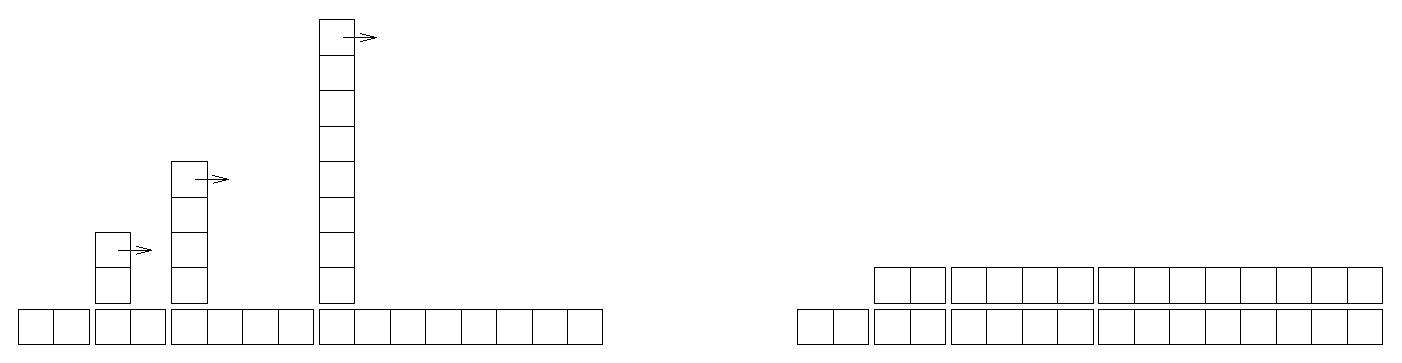
\includegraphics[width=3.0in]{figs/towers}}
\caption{Histogram of wealth with no tax.\label{fig.notax}}
\end{figure}

To compare the effect of taxation on wealth distribution, we need a
metric that measures how distributed or flat a certain wealth
distribution is.  We use the Gini coefficient, which is often used in
economics to measure the wealth gap (see
\url{http://en.wikipedia.org/wiki/Gini_coefficient}). The Gini
coefficient is between 0 and 1, with 0 the measurement of a perfectly
uniform distribution, and 1 the measurement of a distribution with
complete inequality.

Figure~\ref{fig.notax} shows a histogram describing the wealth
distribution when there is no tax system in place. For most initial
conditions without taxation, the Sugarscape quickly develops a
long-tailed distribution of wealth, skewed to the right. In these
cases, some agents die quickly, particularly in an environment with
many agents or one with low sugar regrowth rate. The separation
between the rich and the poor is significant, and there aren't many
agents occupying the middle ground. This is seen in real life in
societies where there is no tax structure and there isn't much of a
middle class.


\section{Reductionism or Holism?}

Written English and Music both share Zipfian properties. A holist would say that Zipf's law is an underlying property of natural languages. What would a reductionist say? Remember that we have reduce language and music alike down too words. This is much the same way a physicist might modle suns and planets like point masses. Can we use this property to make predictions about other natural languages. What would an instrumentalist say? How about a realist?

The construction hypothesis; language and music have these properties because they are constructed.

\begin{figure}[ht]
\centerline{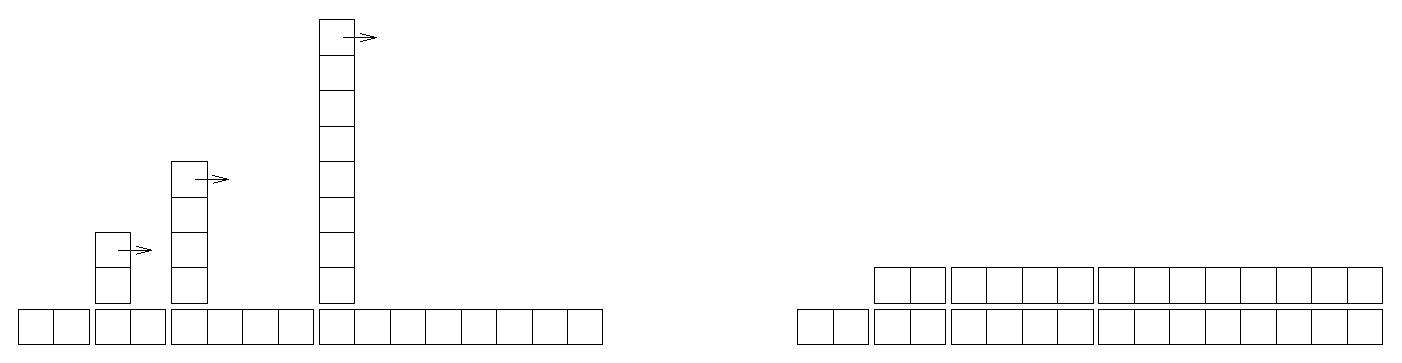
\includegraphics[width=3.0in]{figs/towers}}
\caption{Histogram of wealth, with tax.\label{fig.withtax}}
\end{figure}

\begin{figure}[ht]
\centerline{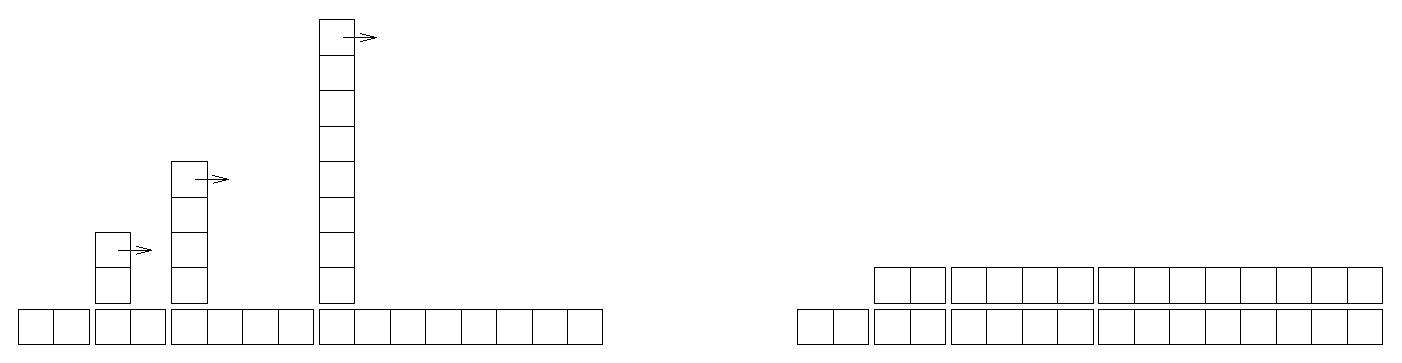
\includegraphics[width=3.0in]{figs/towers}}
\caption{The Gini coefficient versus the tax rate.\label{fig.gini}}
\end{figure}

Figure~\ref{fig.withtax} shows the effect of a relatively high tax
rate. The agents have a similar amount of sugar, and the economy has a
low Gini coefficient, 0.02.

Figure~\ref{fig.gini} shows that
higher taxes in general result in lower Gini coefficients. This makes
sense, since the point of our tax system is to redistribute
wealth.

\begin{figure}[ht]
\centerline{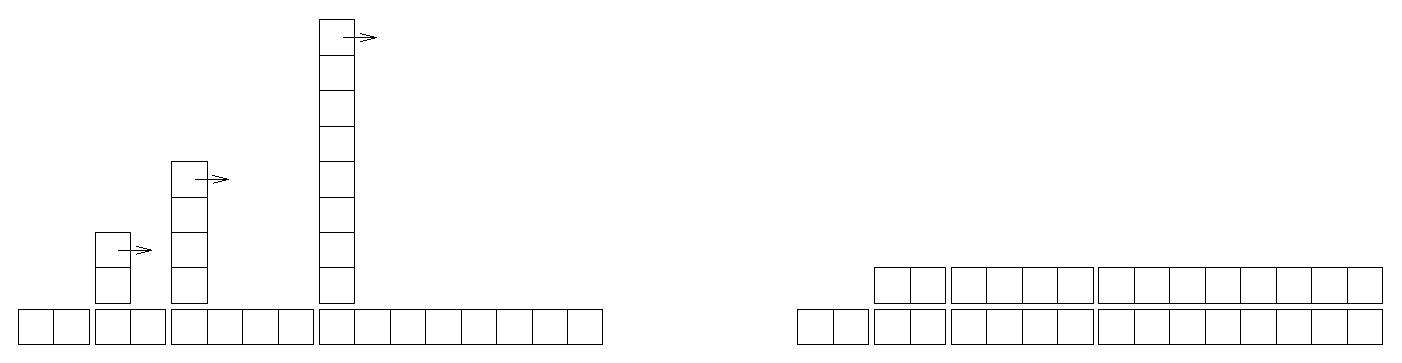
\includegraphics[width=3.0in]{figs/towers}}
\caption{Mean wealth versus tax rate.\label{fig.wealth}}
\end{figure}

In this model, perfect equality comes at a price.  With no taxation
the mean wealth was 358; with a 20\% tax rate it drops to 157.
Figure~\ref{fig.wealth} shows the effect of tax rate on wealth;
mean wealth gets smaller as taxes get higher.



\section{Instrumentalism and Music}

\begin{figure}[ht]
\centering{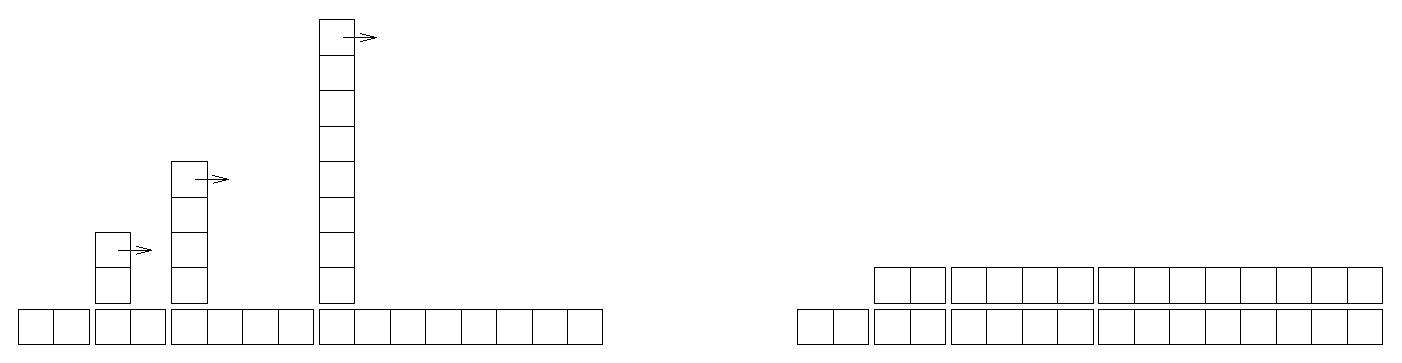
\includegraphics[width=3.0in]{figs/towers}}
\caption{Bottom quartile value versus tax rate. At 4\% the average wealth of the bottom quartile is maximized.\label{fig.optimal}}
\end{figure}

%\begin{figure}[ht]
%\centerline{\includegraphics[width=3.0in]{figs/pmf_2percent.pdf}}
%\caption{The wealth distribution for a smaller tax rate (2\%). There is still s%ome deviation, but the mean wealth is high.}
%\end{figure}

It's up to a society to determine its ideal wealth distribution. 
In our model, there is a conflict between the goals of maximizing
total wealth and minimizing inequality.

One way to reconcile this conflict is to maximize the wealth of
the bottom quartile.  Figure~\ref{fig.optimal} shows the mean
wealth of the poorest 25\% for a range of tax rates.  The optimal
tax rate is around 4\%.  At lower rates, there is more total
wealth, but the poor do not share it.  At higher rates, the poor
have a bigger share of a smaller pie.

Of course, this result depends on the details of our Sugarscape,
especially the model of productivity.  But this simple model
provides a way to explore relationships between wealth creation,
taxation and inequality.

\begin{exercise}

You can download our implementation of Sugarscape from
\url{thinkcomplex.com/Sugarscape.zip}.  Launch it by running
{\tt Gui.py}.  The sliders allow you to control the parameters
of the simulation.  Experiment with these parameters to see what
effect they have on the distribution of wealth.

\end{exercise}

\begin{exercise}

You can download our implementation of Sugarscape from
\url{thinkcomplex.com/Sugarscape.zip}.  Launch it by running
{\tt Gui.py}.  The sliders allow you to control the parameters
of the simulation.  Experiment with these parameters to see what
effect they have on the distribution of wealth.

\end{exercise}

\end{document}
